\documentclass[border=10pt]{standalone}
\usepackage{tikz}

\begin{document}
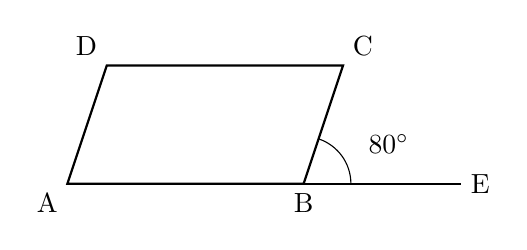
\begin{tikzpicture}[scale=1]
    % Define coordinates for the parallelogram and the extension
    \coordinate (A) at (0,0);
    \coordinate (B) at (3,0);
    \coordinate (C) at (3.5,1.5);
    \coordinate (D) at (0.5,1.5);
    \coordinate (E) at (5,0);

    % Draw the parallelogram segments
    \draw[thick] (D) -- (C) -- (B) -- (A) -- cycle;

    % Draw the extended line segment BE
    \draw[thick] (B) -- (E);

    % Labels for the points
    \node[below left] at (A) {A};
    \node[below] at (B) {B};
    \node[above right] at (C) {C};
    \node[above left] at (D) {D};
    \node[right] at (E) {E};

    % Exterior angle arc and 80 degree label
    \draw (3.6,0) arc (0:71.5:0.6);
    \node[right] at (3.7,0.5) {$80^{\circ}$};
\end{tikzpicture}
\end{document}
